\section{Dataset}
\label{sec:dataset}

In this section, we start by introducing the dataset used for our experiments, then explain how we processed it to use with our model, and finally how we made it an \ac{IID} dataset.
\ \\\\% INPUT DATA
\textbf{\ref{sec:dataset}.1. Input data} 

The dataset we used as starting point is ModelNet10, can be downloaded directly from \textit{https://modelnet.cs.princeton.edu/}. It contains 4899 3D CAD models divided into 10 different categories and has an initial splitting of the data into 80\% for training and 20\% for testing.
Fig.~\ref{fig:CADModels} shows some examples of chairs and monitors in the dataset.

% CAD Models
% \begin{figure}[h]
%     \begin{center}
%         \centering
%          \begin{subfigure}[b]{0.42\textwidth}
%              \centering
%              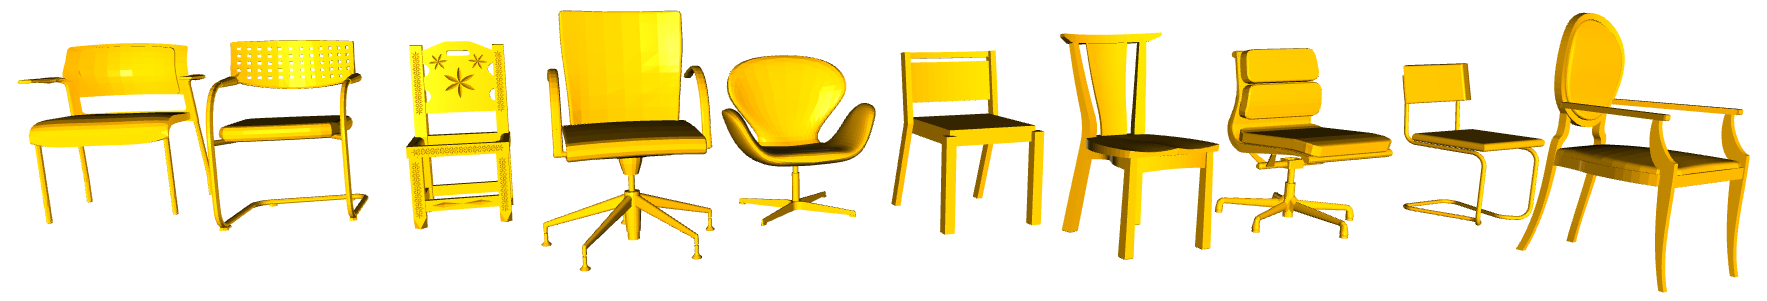
\includegraphics[width=\textwidth]{resources/chairs.png}
%              \caption{Chairs}
%              \label{fig:chairs}
%          \end{subfigure}
%          \begin{subfigure}[b]{0.42\textwidth}
%              \centering
%              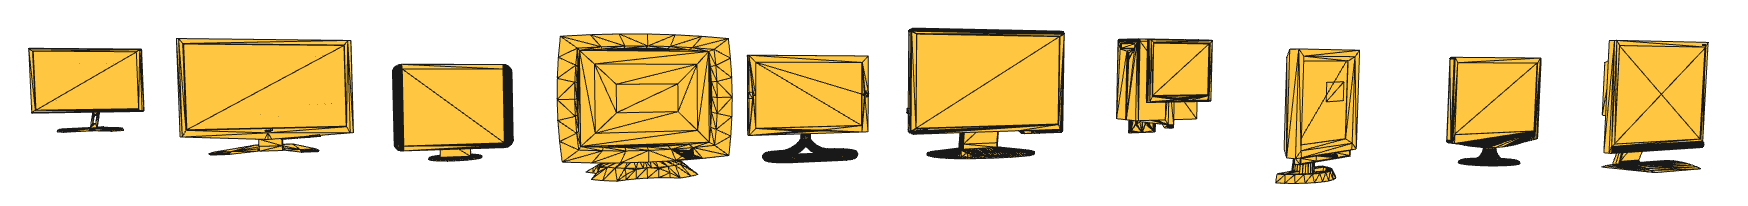
\includegraphics[width=\textwidth]{resources/monitor.png}
%              \caption{Monitors}
%              \label{fig:monitors}
%          \end{subfigure}
%         \caption{Example of (a) Chairs and (b) Monitors samples from ModelNet10 dataset.}
%         \label{fig:CADModels}
%     \end{center}
% \end{figure}
% % Voxelized Models
% \begin{figure}[h]
%     \begin{center}
%         \centering
%          \begin{subfigure}[b]{0.42\textwidth}
%              \centering
%              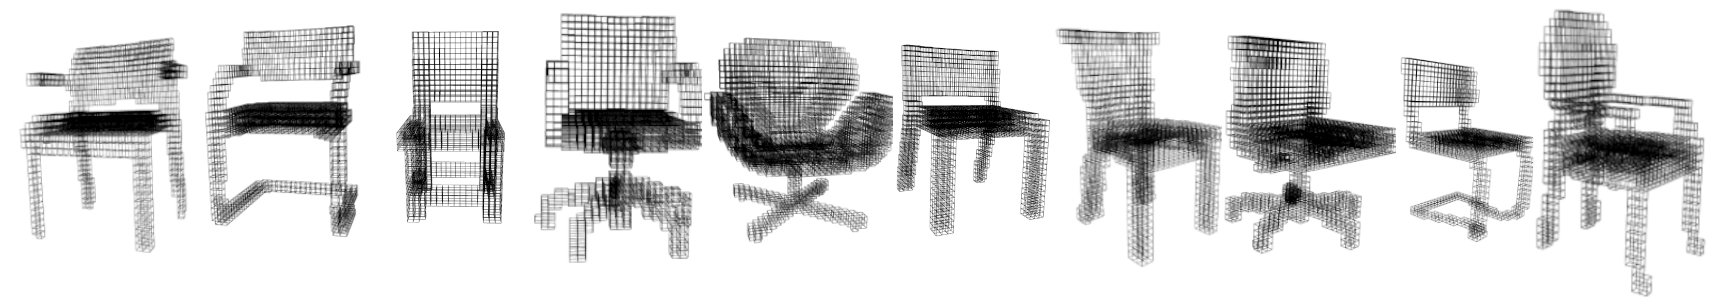
\includegraphics[width=\textwidth]{resources/chairs_voxels.png}
%              \caption{Chairs}
%              \label{fig:chairs}
%          \end{subfigure}
%          \begin{subfigure}[b]{0.42\textwidth}
%              \centering
%              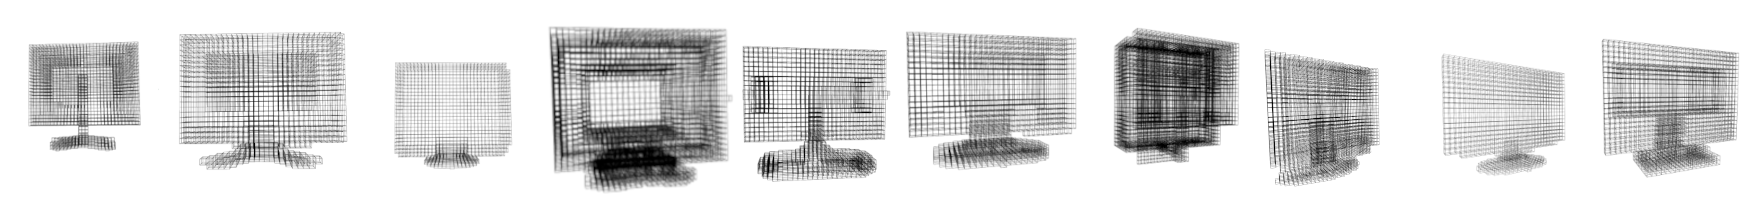
\includegraphics[width=\textwidth]{resources/monitors_voxels.png}
%              \caption{Monitors}
%              \label{fig:monitors}
%          \end{subfigure}
%         \caption{Example of voxelized (a) Chairs and (b) Monitors samples of Figure \ref{fig:CADModels}}
%         \label{fig:VoxelizedModels}
%     \end{center}
% \end{figure}
\ \\ % PRE-PROCESSING DATA
\textbf{\ref{sec:dataset}.2. Pre-processing data}

We had to solve mainly 2 problems with the initial dataset:
\begin{itemize}
    \item the samples were 3D CAD Models, so we needed to convert them into voxel grids for our needs;
    \item as we already mentioned, the Dataset is not \ac{IID}, so we decided to augment with rotations to make the categories well-balanced, Fig.~\ref{fig:finalTrainSetDistribution} in blue shows the initial dataset distribution of the Train folder.
\end{itemize}
%\ \\% 1)
\textbf{\ref{sec:dataset}.2.1. Voxelization}

The CAD models are Meshes, see Fig.~\ref{fig:CADModels} for reference, in Object File Format (OFF) but our model, described in the Sec.~\ref{sec:learning_framework}, requires 3D boolean vectors with dimensions of \mbox{$32\times32\times32$}.

With the help of the Open3d Python library \cite{Zhou2018}, we converted all the meshes into voxel grids after scaling them. 
% The code is available in our Git repository under the folder:  \mbox{\textit{code/preprocessing/voxelization/}}. \\
As mentioned before, voxel grids of size \mbox{$32\times32\times32$} are a good compromise between memory and information loss, and in our case we went from 2.17 GB of CAD models to 311 MB in voxelized version. 

Fig.~\ref{fig:VoxelizedModels} shows the voxelized samples of Fig.~\ref{fig:CADModels}.

We opted to store the normalized voxel grids directly on disk to reduce computation time during the training phase, as we relied only on the free tiers of GPU provided by Google Colab and Kaggle.\\
\ \\\\% 2)
\textbf{\ref{sec:dataset}.2.2. Data Augmentation}

The unbalanced distribution of the dataset may cause models to overfit classes with more samples, thus lowering the performances. 
Furthermore, in a real-world scenario, we found it very useful to consider that the model should be rotation-invariant, meaning that it can recognize objects regardless of their rotation.
Keeping in mind the above and the need to create a robust system, we choose to augment the data with new the rotation along the vertical axis. 

The rotations were made by adding multiples of 30 degrees to the initial orientation, thus in total we could have 12 possible rotations. Fig.~\ref{fig:rotatedChair} shows all the possible rotations of the first chair in Fig.~\ref{fig:chairs}.
% Rotated Models
\begin{figure}[h]
\begin{center}
        \centering
        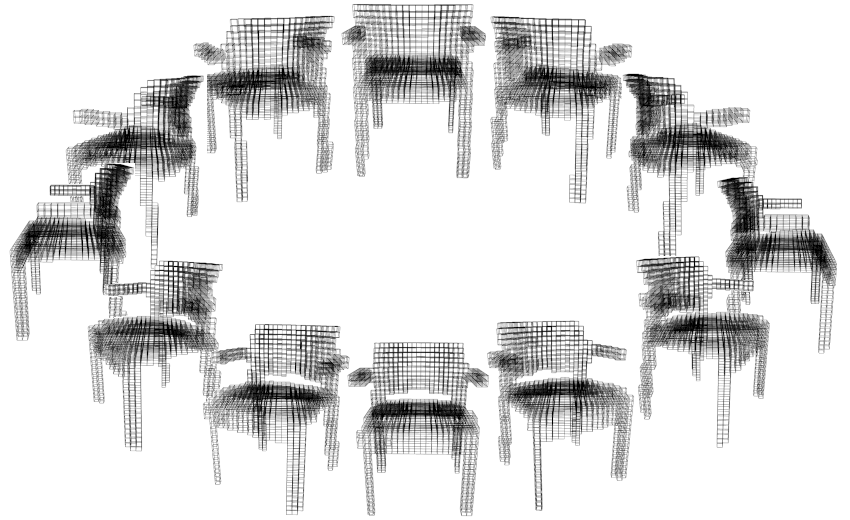
\includegraphics[width=0.42\textwidth]{resources/rotated_voxels_2.png}
        \caption{Example of possible rotation of the first Chairs in Figure \ref{fig:chairsVoxels}}
        \label{fig:rotatedChair}
    \end{center}
\end{figure}
In order to make the classes as equally distributed as possible, we choose uniformly at randomly N different rotations from all the possible ones. N values for each model in Train folder are described in Tab.~\ref{tab:modelRotations}. Meanwhile, we set N = 3 for the Test folder.

\begin{table}[h]
	\centering
	\caption{Categories and their N for Train partition, N is the total number of selected rotations}
	\label{tab:modelRotations}
	\begin{tabular}{|c||c|}
		\hline
		Rotations & Models \\
		\hline
		\hline
            2 & bed, chair, monitor, sofa\\\hline
            3 & table, toilet\\\hline
            5 & desk, dresser, night_stand\\\hline
            8 & bathtub\\\hline
	\end{tabular}
\end{table}

Fig.~\ref{fig:finalTrainSetDistribution} shows in orange the distribution after the Data augmentation.


% TODO: Also on Test set?
\begin{figure}[h]
\begin{center}
        \centering
        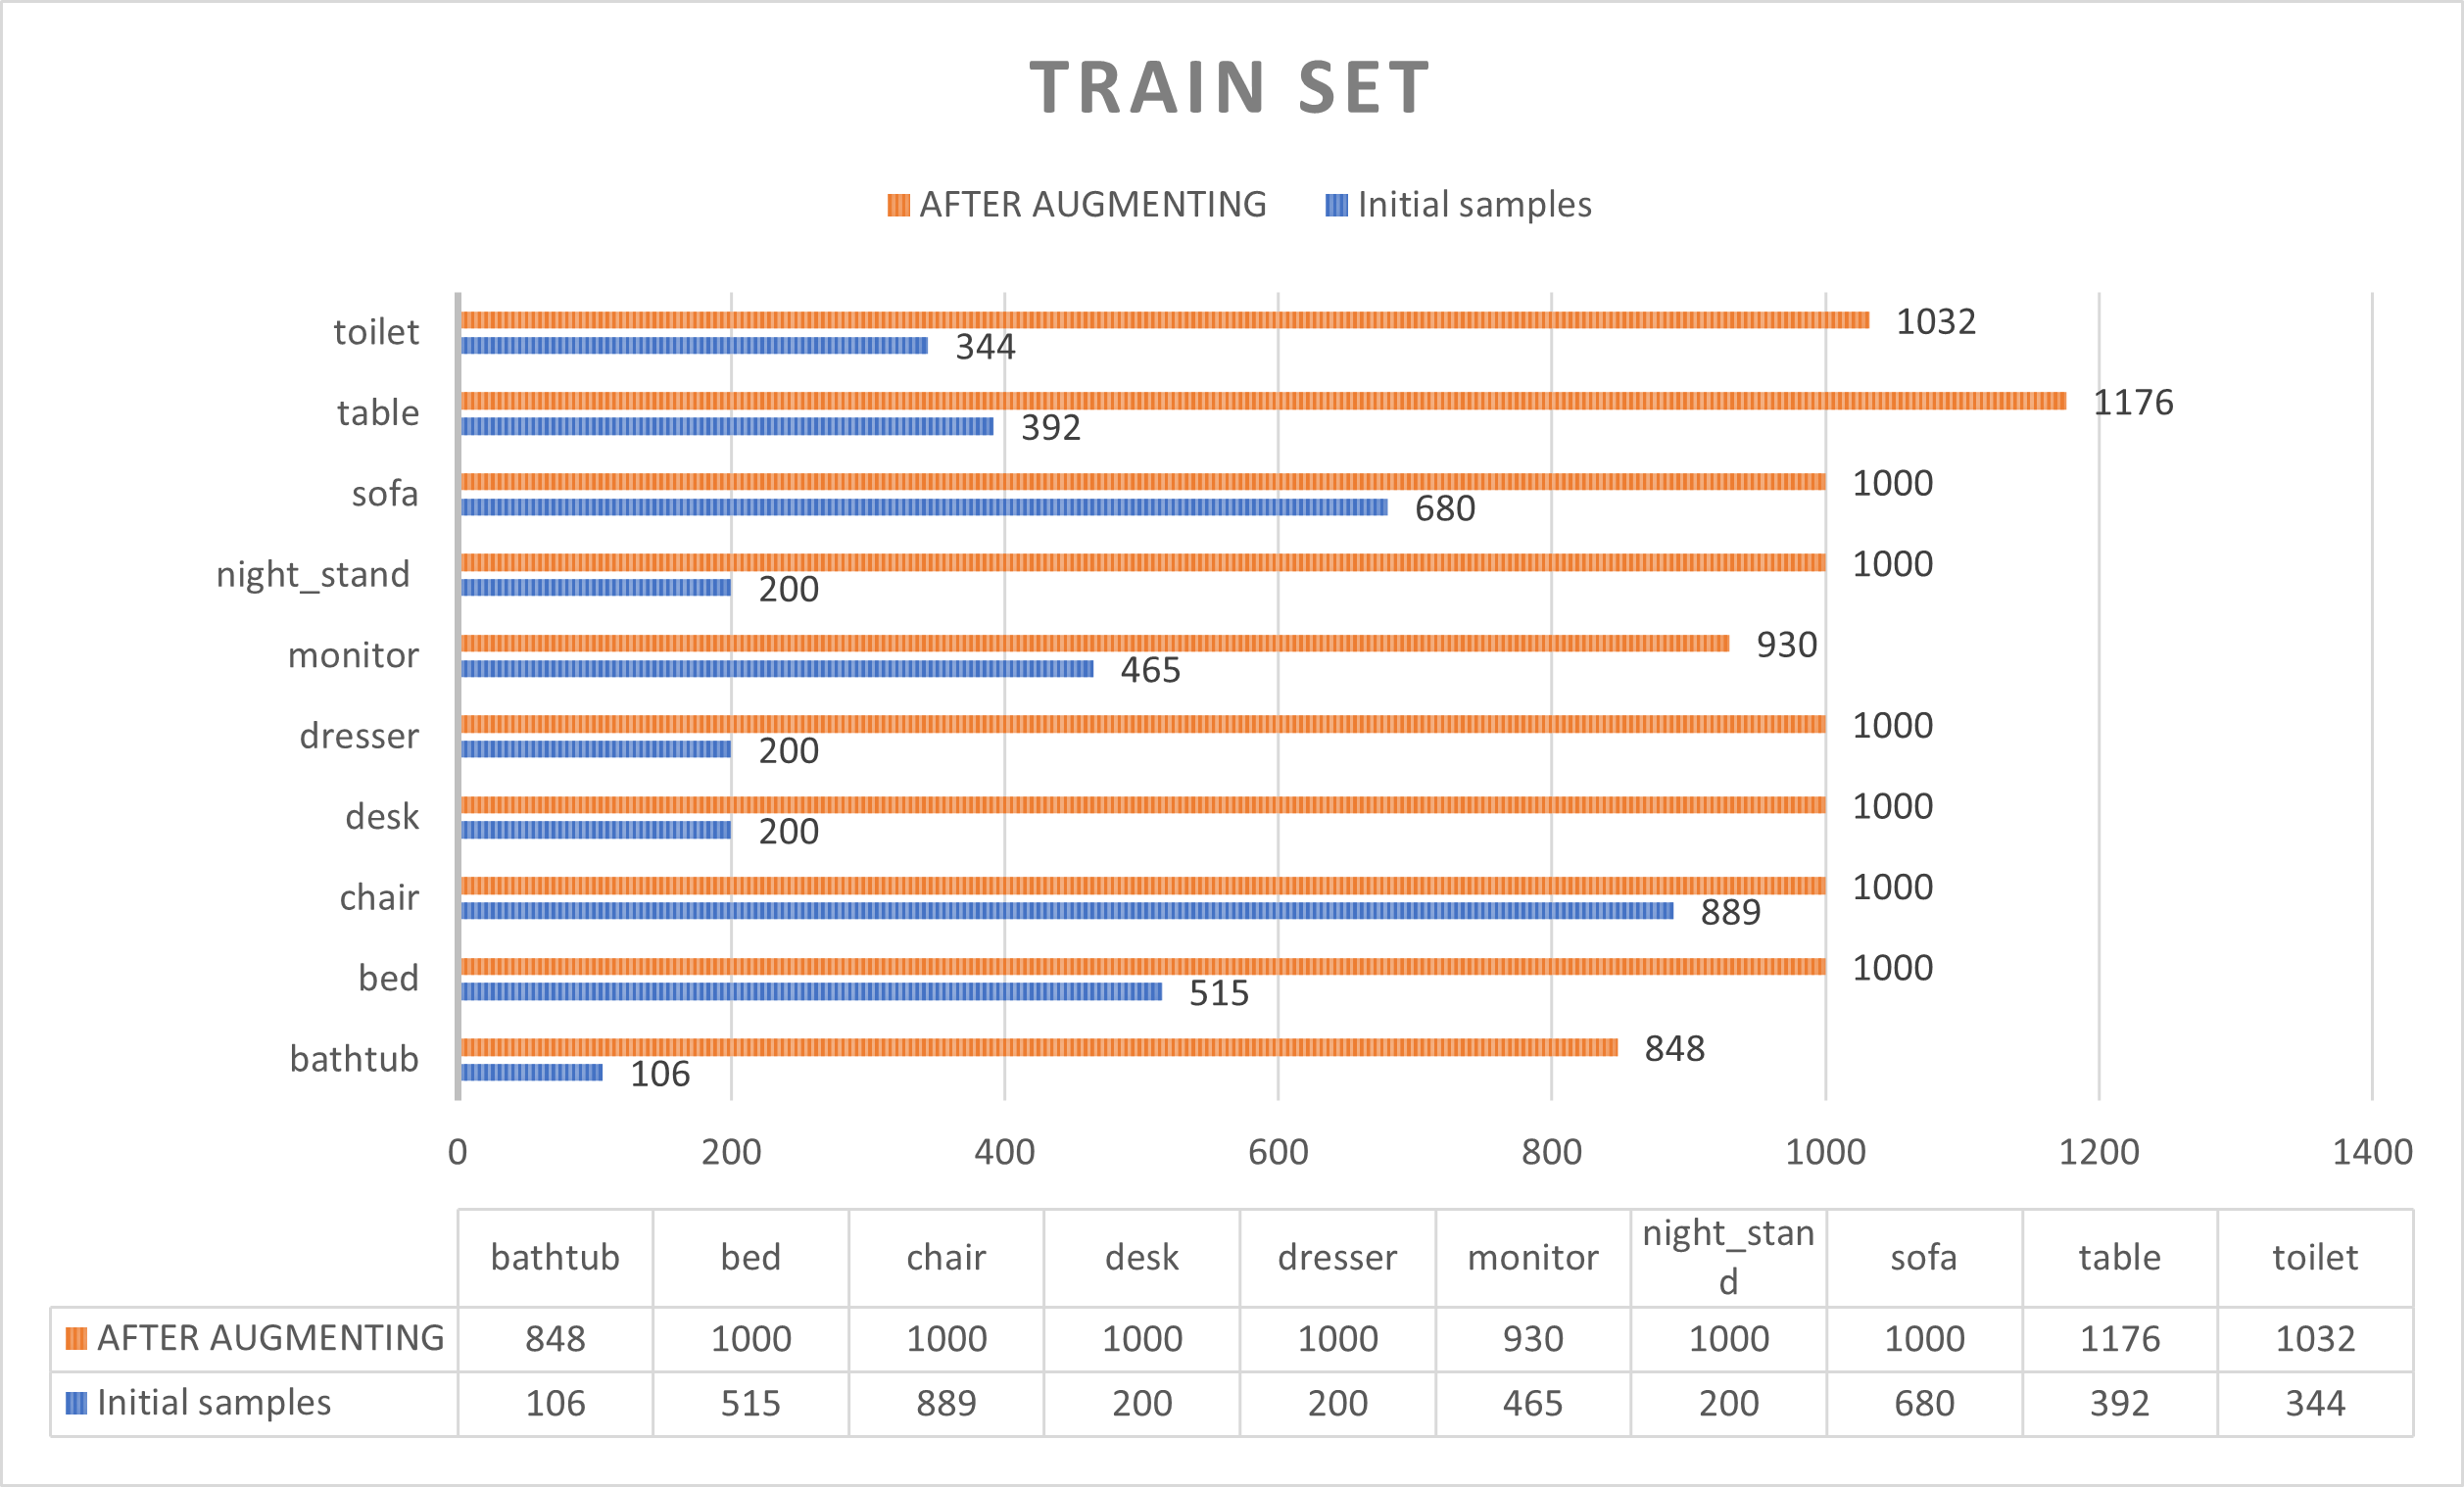
\includegraphics[width=0.42\textwidth]{resources/finalTrainDistribution.png}
        \caption{Distributions Before (in blue) and After (in orange) the data augmentation}
        \label{fig:finalTrainSetDistribution}
    \end{center}
\end{figure}

% As we can see from Figure \ref{fig:initialTrainSetDistribution}, the ModelNet10 is not an Independent and Identically Distributed (i.i.d.) dataset. The assumption of I.I.D is central to almost all machine learning algorithms, and we tried to make our data as much as i.i.d in the following way:
% \begin{itemize}
% 	\item Firstly, we normalized the data, from the previous step, by subtracting the mean and dividing by the standard deviation. [TODO: remove?]
% 	\begin{center}
% 		\textit{
% 			normalized\_voxelgrid = (voxelgrid - mean) / std
% 		}
% 	\end{center}
	
% 	\item Then, we augmented the dataset with new rotations of the voxel grids. Rotations are made by adding multiples of 30 degrees to the initial orientation. [TODO with formulas?]
	
% 	\item Finally, we randomly picked, per category, $\sim$1k samples for the train set and $\sim$300 samples for the test set. [TODO we are not precise here]
	
% \end{itemize}
% Figure \ref{fig:finalTrainSetDistribution} shows the distribution we get after these steps.
\ \\ % PARTITIONING DATA
\textbf{\ref{sec:dataset}.3. Partitioning data}

% A good practice is to divide the dataset into three sets: one set for training and two smaller sets for validation and testing.
% The ratio we used for splitting is 80/10/10, where 80 percent of the data is put into the training set, and the remaining percentage is equally spread across the test and validation sets.
To train the weak models for the bagging classifier, see Sec.~\ref{sec:learning_framework}, we created five different subsets with custom rules. 
The intention was to make each weak model :
\begin{itemize}
    \item learn well from their part of the dataset (chunk),
    \item also learn some information from the data of other models.
\end{itemize}

In details, we:
\begin{enumerate}
    \item Split tidily the rotated dataset into 25 subsets;
    \item Created 5 initial ordered chunks from the subsets;
    \item Copied each subset, of each chunk, into a different dataset w.r.t the initial chunk's dataset.
\end{enumerate}

 Tab.~\ref{tab:partitions} shows possible permutations for the datasets.

\begin{table}[h]
	\centering
	\caption{Our Bagging datasets compositions}
	\label{tab:partitions}
	\begin{tabular}{|c||c|c|}
		\hline
		Dataset & Chunk's subsets & Copied Subset \\
		\hline
		\hline
            1 & \small{01, 02, 03, 04, 05} & \small{10, 15, 20, 25 | 24}\\\hline
            2 & \small{06, 07, 08, 09, 10} & \small{01, 11, 16, 21 | 05}\\\hline
            3 & \small{11, 12, 13, 14, 15} & \small{02, 07, 17, 22 | 06}\\\hline
            4 & \small{16, 17, 18, 19, 20} & \small{03, 08, 13, 23 | 12}\\\hline
            5 & \small{21, 22, 23, 24, 25} & \small{04, 09, 14, 19 | 18}\\\hline
	\end{tabular}
\end{table}


\textbf{\ref{sec:dataset}.4. CutOut}

Finally, as explained in Chapter 3, we will perform the cutout on a portion of the dataset, masking out a random 8x8x8 portion of the input data. The probability that the cutout is applied to each sample is 20\%.